\scanpage{22}
\hfill\handwritten{\unsure{Massy} 22. 10. 1969}\\

Dear Kostant,\\

I read again through your papers in the \unsure{Maer.|Amer.} Journ. on \handwritten{``}\deleted{t}\handwritten{T}he principal three-dimensional subgroup ...\handwritten{''} and \handwritten{``}Lie group representations on polynom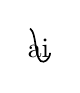
\begin{tikzpicture}[baseline=(letters.base),x=1em,y=1em]
\node[inner sep=0pt] (letters) at (0,0) {ai};
\handwritten{\draw[line width=.6pt] (-.30,.72) .. controls (-.04,.55) and (-.16,-.55) .. (.19,-.48) .. controls (.34,-.46) and (.44,-.22) .. (.42,-.16);}
\end{tikzpicture}l rings\handwritten{''}, prompted by some nice work of Brieskorn on Klein singularities. I very much appreciate this work of yours, and would appreciate getting reprints of any later work you may have available. As I already felt when your work appea\unsure{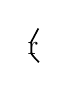
\begin{tikzpicture}[baseline=(appeared.base),x=1em,y=1em]
\node[inner sep=0pt] (appeared) at (0,0) {r};
\handwritten{\draw[line width=.6pt] (-.08,.22) -- (.19,.73);
\draw[line width=.6pt] (-.06,-.18) .. controls (.03,-.32) and (.13,-.40) .. (.21,-.49);}
\end{tikzpicture}}ed, it cries for careful reconsideration in the framework of \deleted{\unsure{a|A}}\handwritten{A}lg. Geometry, and suggests number of interesting problems. I wonder if you know the answer to some of them. For instance, I feel it would be of interest to classify (for a given complex simple adjoint Lie group, say) quadr\deleted{\unsure{a|u}}uples $(\mathrm{T},\mathrm{B},\mathrm{T}',\mathrm{B}')$, where $\mathrm{T}$ and $\mathrm{T}'$ are maximal tori ``in apposition\handwritten{''} (in your terminology), and $\mathrm{B}$ and $\mathrm{B}'$ Borel subgroups of $\mathrm{G}$ containing $\mathrm{T}$ resp. $\mathrm{T}'$. The number of conjugacy classes of such animals is equal to $\operatorname{card}(\mathrm{W})^{2}/\mathrm{hz}\handwritten{\phi}(\mathrm{h})$, where $\deleted{\unsure{\mathrm{H}|\mathrm{W}}}\handwritten{W}$ is the Weyl group, $\mathrm{h}$ the Coxeter number, $\mathrm{z}$ the order of the center\inserted{\handwritten{of $\widetilde{G}$}}, and $\handwritten{\phi}(\mathrm{h})=\operatorname{card}(\underline{\mathrm{Z}}/\mathrm{h}\underline{\mathrm{Z}})^{\handwritten{*}}$ is the Euler indicatrix; if you want to classify such data with moreover a\deleted{n} \inserted{generating} element (principal regular in your terminology) given for the finite group of order $\mathrm{h}$ $\mathrm{T}\handwritten{\cap}\mathrm{N}(\mathrm{T}')$, then we get $\operatorname{card}(\mathrm{W})^{\handwritten{2}}/\mathrm{hz}$ choices. One of the reasons I think this question is interesting is that the stablity subgroup in $\mathrm{G}$ of such a quadruple is $\mathrm{T}\handwritten{\cap}\mathrm{T}'=\mathrm{e}$,\handwritten{\textsuperscript{*}} hence such a structure makes $\mathrm{G}$ entirely ``rigid'' up to exterior automorphisms. Among the first questions one may wish to ask in this direction are the following: is it true that for some, or for all, such quadruples, $\mathrm{B}$ and $\mathrm{B}'$ are ``in general position'' i.e. $\mathrm{B}\handwritten{\cap}\mathrm{B}'$ is a torus (necessarily maximal), so that $\mathrm{B}$ and $\mathrm{B}'$ are ``opposite'' to each other with respect to the latter ? Is there in any sense a \uline{distinguished} conjugacy class of such quadruples (which should then be, of course, invariant by action of exterior automorphisms) ? What are the groups of automorph\unsure{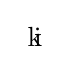
\begin{tikzpicture}[baseline=(automorph.base),x=1em,y=1em]
\node[inner sep=0pt] (automorph) at (0,0) {k};
\node[inner sep=0pt] at (.11,0) {i};
\end{tikzpicture}}sms of such quadr\deleted{a}uples (they

\margin{\handwritten{* NB: $N(T)\cap N(T')$ is an extension of $(\mathbb{Z}/h\mathbb{Z})^{*}$ by $\mathbb{Z}/h\unsure{Z|\mathbb{Z}}\times$ 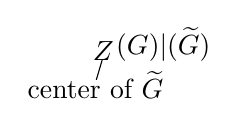
\begin{tikzpicture}[baseline=(centerZ.base),x=1em,y=1em]
\node[inner sep=0pt] (centerZ) at (0,0) {$Z$};
\node[anchor=base west,inner sep=0pt] at (.45,-.14) {$\deleted{\unsure{(G)|(\widetilde{G})}}$};
\draw[line width=.4pt] (-.04,-.34) -- (-.25,-1.05);
\node[anchor=base west,inner sep=0pt] at (-2.75,-1.72) {center of $\widetilde{G}$};
\end{tikzpicture}, 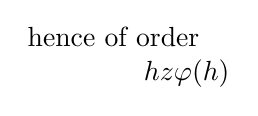
\begin{tikzpicture}[baseline=(order.base),x=1em,y=1em]
\node[anchor=base west,inner sep=0pt] (order) at (0,0) {hence of order};
\node[anchor=base west,inner sep=0pt] at (4.2,-1.22) {$hz\varphi(h)$};
\end{tikzpicture}}}
% Bottom margin note. Its center annotation lies below and to the left of Z;
% its final order formula is written on a lower row towards the right edge.
% The appeared and automorphisms cells retain overlapping contours without assigning chronology.
% The handwritten transposition stroke crosses the original typed ``ai'' in ``polynomail''.
% archive sheet number: 21
